\documentclass[12pt,a4paper]{article}
% Set paper dimension
\usepackage[
  top=2cm,
  bottom=2cm,
  left=2cm,
  right=2cm,
  headheight=17pt, % as per the warning by fancyhdr
  includehead,includefoot,
  heightrounded, % to avoid spurious underfull messages
]{geometry}
\usepackage[english]{babel}
\usepackage[utf8]{inputenc}
\usepackage{graphicx}
\graphicspath{ {images/} }
\usepackage{amsmath}
\usepackage{mathtools}
\usepackage{amsfonts}
\usepackage{amssymb}
\usepackage{fancyhdr}
\usepackage{wrapfig}
\usepackage{lscape}
\usepackage{rotating}
\usepackage{epstopdf}
%\usepackage{glossaries}
\usepackage{float}
\usepackage{titlesec}
\usepackage{paralist}
% Index
\usepackage{makeidx}
\makeindex
\usepackage[nottoc]{tocbibind}


\usepackage{multicol}

\makeindex
%makeindex -s format.ist myfile.idx
\title{Software Design Document}

% For the revision table
\usepackage[table]{xcolor}
\setlength{\arrayrulewidth}{0.5mm}
\setlength{\tabcolsep}{12pt}
\renewcommand{\arraystretch}{1.5}
\renewenvironment{enumerate}[1]{\begin{compactenum}#1}{\end{compactenum}}

\usepackage{hyperref}
 % Margins
\topmargin=-0.1in

% Headings
\pagestyle{fancy}
\fancyhf{}
\rhead{\textbf{Page} \thepage}
\lhead{User Manual for Lunar Rover Mapping Robot}

\pagenumbering{roman}

\begin{document}
	\begin{titlepage}
		\centerline{\rule{6.5in}{4pt}}
		\vspace*{0.5in}
		\begin{center}
			{\fontfamily{cmr}\selectfont
				{\fontsize{33}{40}\selectfont \textbf{User Manual}}\\
				\vspace*{0.5in}
				{\fontsize{20}{40}\selectfont for}\\
				\vspace*{0.5in}
				{\fontsize{33}{40}\selectfont \textbf{Lunar Rover Mapping Robot}}\\
				\vspace*{0.65in}
				{\fontsize{18}{40}\selectfont Version 1.0}\\
				\vspace*{2.5cm}
				{\fontsize{25}{40}\selectfont \textbf{Group: UG12}}\\
				\vspace*{2.5cm}
                \begin{figure}[H]
                \centering
                
\includegraphics[width=0.5\textwidth]{UofA.jpg}
              \end{figure}
              \vspace*{\fill}
			}
		\end{center}
		\centerline{\rule{6.5in}{4pt}}
	\end{titlepage}

	\newpage

	\tableofcontents

    \newpage

	\noindent{\fontsize{16}{40}\textbf{Revision History}}
	\begin{center}
	\begin{tabular}{ |p{2cm}|p{3cm}|p{9cm}|  }
	\hline
	\rowcolor{lightgray}
	Version & Date &Reason for changes \\
	\hline
	1.0 & 28/10/2017 &Final version \\
	\hline
	\end{tabular}
	\end{center}

    \vspace{50px}
    \listoffigures

	\newpage

    	\pagenumbering{arabic}


\section{Overview}

\subsection{Introduction}
	This document is a user guide for use of Lunar Rover Mapping Project and provide guidance on both the robot and server side. The document also provide necessary information for user to deal with some frequent problem that may occur during the operation.
\subsection{System Requirement}
Before we get started, the following describe the necessary requirements to run the application. \\ 
\newline
\textbf{Computer requirements} \index{Computer Requirements}
	\begin{itemize}
	\item WiFi
    \item Bluetooth
    \item At least 500MB of RAM
    \item At least 200MB of HDD
    \item Java 7
    \end{itemize}
\textbf{Robot Requirement} \index{Robot Requirement}
	\begin{itemize}
    \item Robot EV3 Brick
    \item EV3 Ultrasonic sensor
    \item EV3 Gyro sensor
    \item Color Sensor
    \item EV3 Motors
	\item USB WiFi adapter
    \end{itemize}

\subsection{Definitions, Acronyms, and Abbreviations}
\begin{itemize}
\item CPU: Central Processing Unit
\item GPU: Graphics Processing Unit
\item GUI: Graphical User Interface
\item HDD: Hard Disk Drive
\item RAM: Random Access Memory
\item UI: User Interface
\end{itemize}


\newpage
\section{Robot EV3}
\subsection{EV3 Brick} \index{EV3 Brick Setup}
The EV3 Brick (Figure \ref{brick}) is the control center and power station for the robot. All sensors and motors must be connected to the EV3 brick before starting the application. To start the brick, hold the center button for 2 to 3 sec and "leJOS EV3" will be displayed on the brick screen. The booting normally needs around 110 sec. \\
\begin{figure}[!htb]
\centering
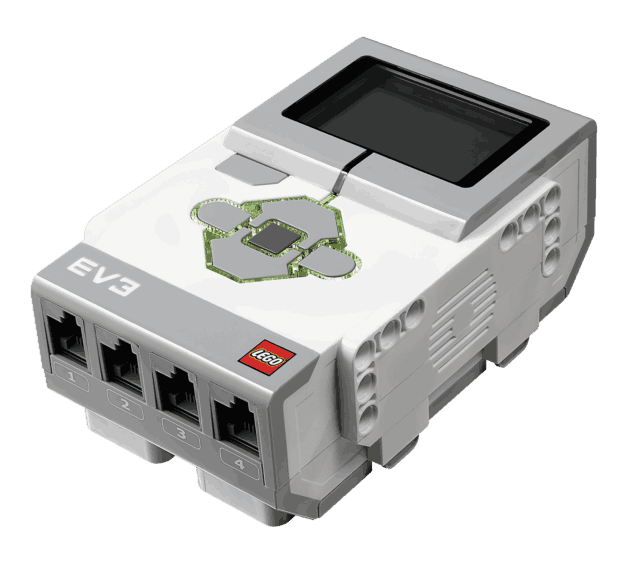
\includegraphics[width=0.2\textwidth]{Ev3Brick.png}
\caption{Ev3 Brick}
\label{brick}
\end{figure}

\subsection{Color Sensor} \index{Color Sensor}
The color sensor (Figure \ref{color}) recognizes the different colors and measures light intensity. The application requires the color sensor to be connected to port 1 of the brick. Otherwise, the application will fail to set up the color sensor.
\begin{figure}[!htb]
\centering
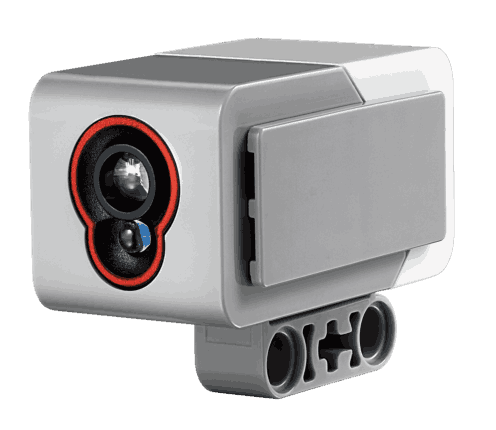
\includegraphics[width=0.2\textwidth]{ColorSensor.png}
\caption{Color Sensor}
\label{color}
\end{figure}

\subsection{Gyroscopic Sensor} \index{Gyroscopic Sensor}
The EV3 Gyro Sensor (Figure \ref{gyro}) measures the robot’s rotational motion. The application requires the Gyro Sensor to be connected to port 4 of the brick. Otherwise, the application will fail to set up the Gyro Sensor.
\begin{figure}[!htb]
\centering
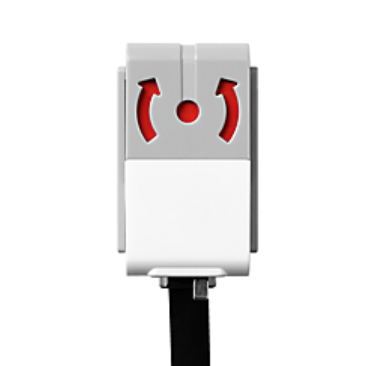
\includegraphics[width=0.2\textwidth]{GyroSensor.png}
\caption{Gyro Sensor}
\label{gyro}
\end{figure}
\newpage
\subsection{Large Motors}\index{Large Motors}
Large Motors (Figure \ref{large motor}) controls the movement of the robot. The application requires the left motor to be connected to port D and the right motor connected to port A. Otherwise,the application will fail to set up the motors.
\begin{figure}[!htb]
\centering
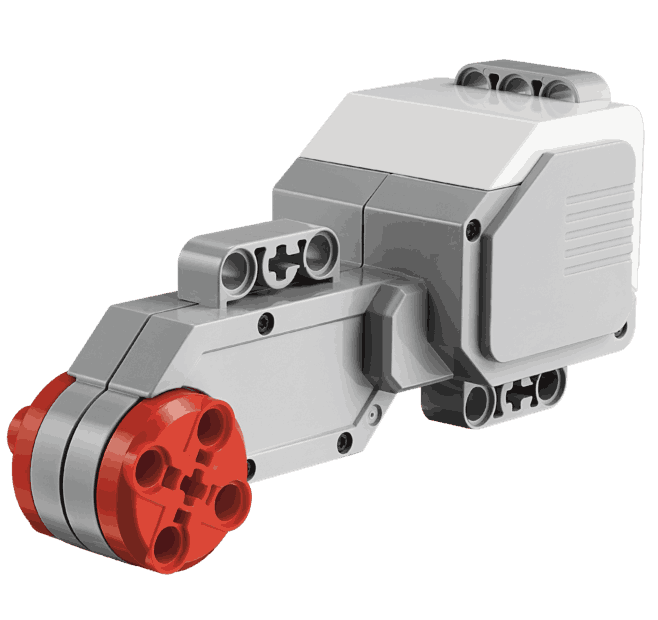
\includegraphics[width=0.2\textwidth]{LargeMotor.png}
\caption{Large Motor}
\label{large motor}
\end{figure}

\subsection{Medium Motor} \index{Medium Motor}
In this application, the Medium Motor (Figure \ref{medium motor}) control the movement of color sensor. The application requires it to be connected to port C. Otherwise,the application will fail to set up the Medium Motor.
\begin{figure}[!htb]
\centering
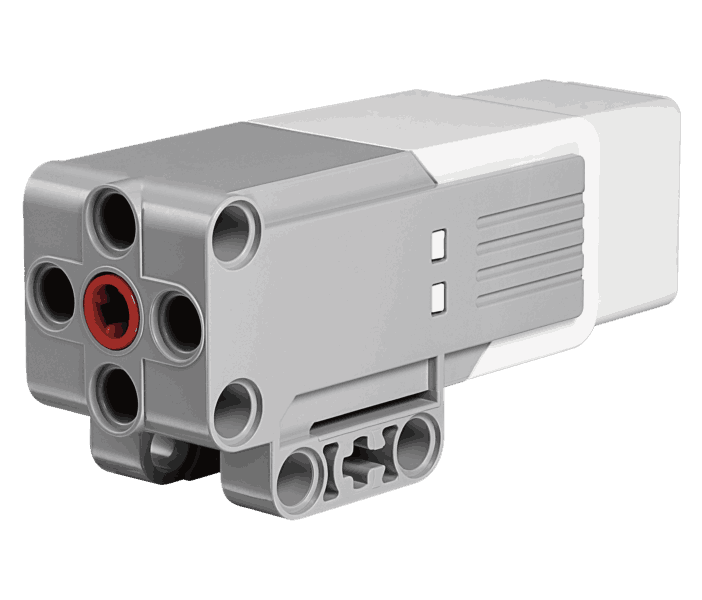
\includegraphics[width=0.2\textwidth]{MediumMotor.png}
\caption{Medium Motor}
\label{medium motor}
\end{figure}

\newpage
\section{GUI}
On the server side, the Lunar Rover Mapping Project includes a GUI that provides a window to allow the user to interact with the application. The GUI has two screens: a connection screen, and a main screen. The connection screen will pop out at the launch of application. The main screen will only displayed after the connection is successfully built.

\subsection{Connection screen} \index{Connection Screen}
The connection screen (Figure \ref{connection screen})  is comprised of two sections. The message window displays the setting up information for each senor and motor. The selection panel is used for selecting the connection method.
\begin{figure}[!htb]
\centering
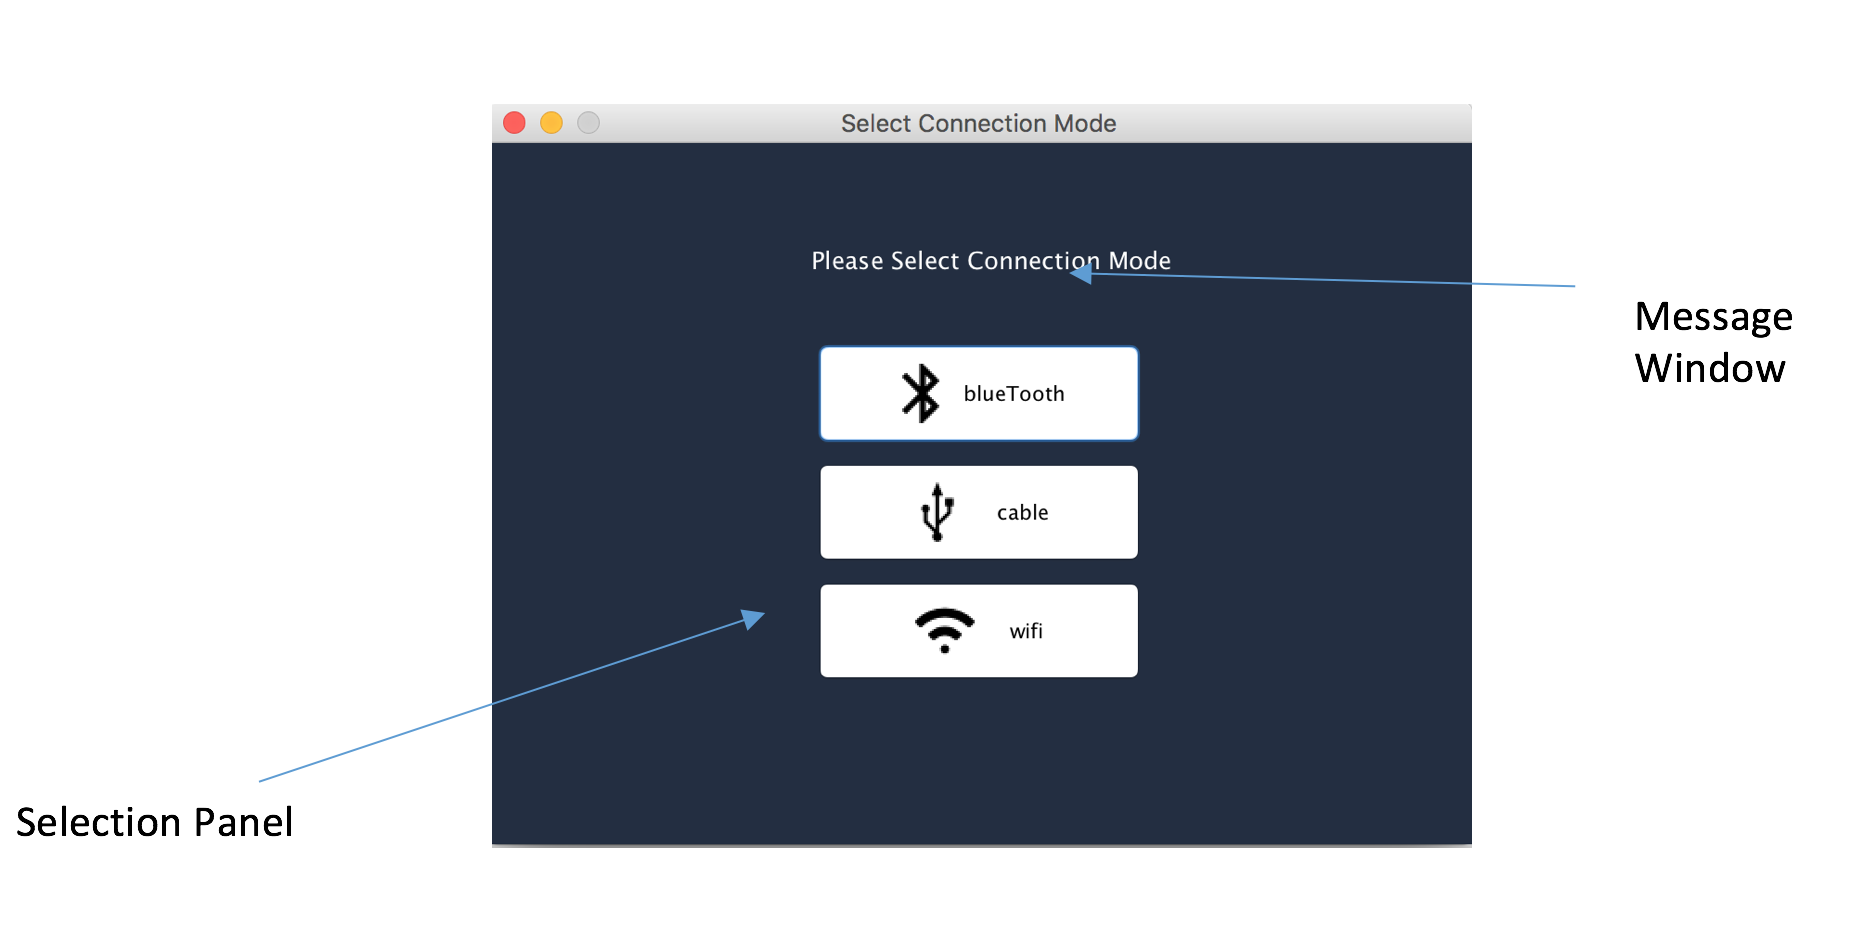
\includegraphics[width=0.8\textwidth]{ConnectionScreen.png}
\caption{Connection Screen}
\label{connection screen}
\end{figure}

\begin{itemize}
\item "Bluetooth" button should be selected when the connection is via Bluetooth. The robot will have the IP address 10.0.1.1. \index{Bluetooth Connection Information}
\item "Cable" button should be selected when the connection is via a USB cable. The robot will have the IP address 10.0.1.1. \index{Cable Connection Information}
\item "WiFi" button should be selected when the connection is via WiFi. The robot will be assigned an IP address and it is displayed on the brick screen. It will pop up a prompt to ask the user to enter the IP address. \index{WiFi Connection Information}
\end{itemize}
\newpage
\subsection{Main Screen} \index{Main screen}
The layout of the main screen (Figure \ref{main screen}) is comprised of the following sections: the control panel, switch panel, and map display region. The control panel provides buttons that allow the user to manually control the movement of the robot. The switch panel provides buttons to switch between the manual and autonomous mode of the robot, and clear the map creations e.g. destinations. The map display region renders the map structure and presents a graphical representation of the map to user. \\
\\
\begin{figure}[!htb]
\centering
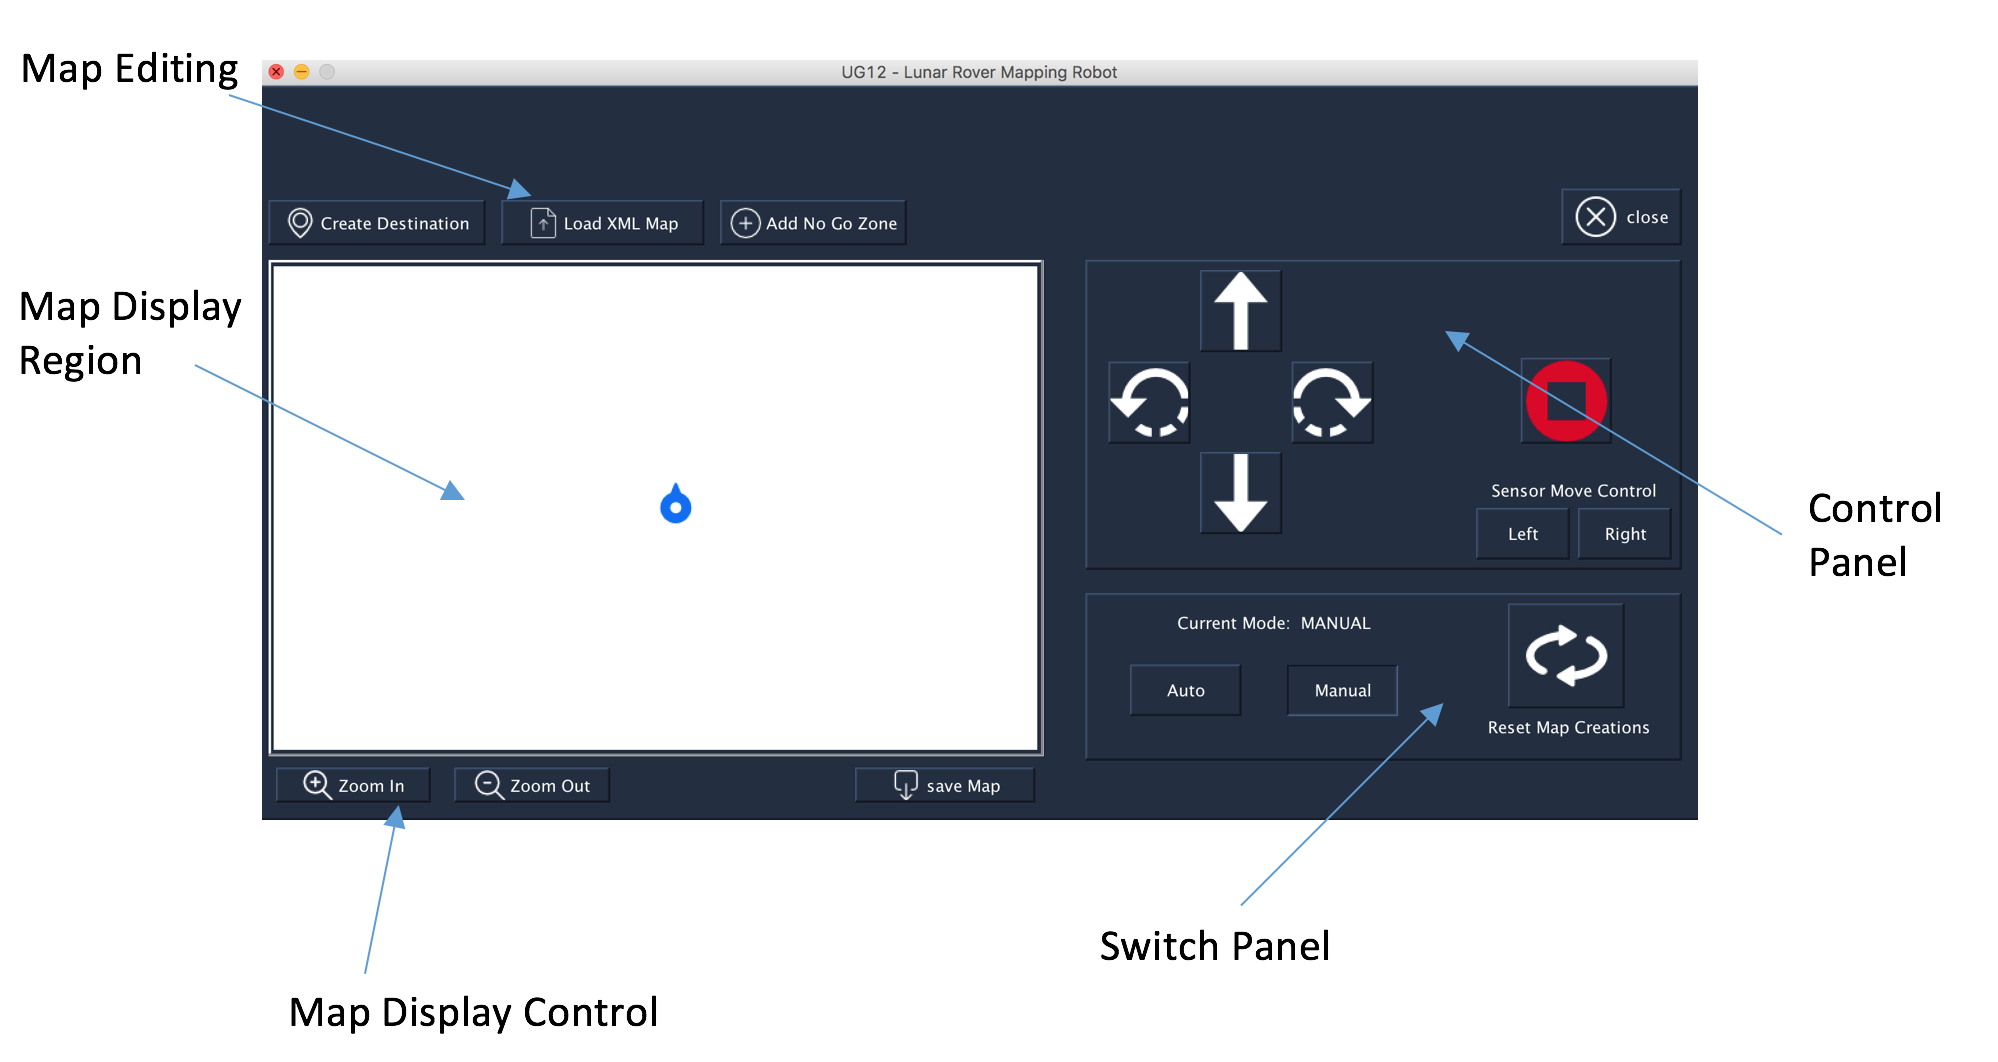
\includegraphics[width=0.8\textwidth]{GUILayout.png}
\caption{Main Screen}
\label{main screen}
\end{figure}

\setcounter{secnumdepth}{4}

\titleformat{\paragraph}
{\normalfont\normalsize\bfseries}{\theparagraph}{1em}{}
\titlespacing*{\paragraph}
{0pt}{3.25ex plus 1ex minus .2ex}{1.5ex plus .2ex}


\subsubsection {Control Panel} \index{Control Panel}
\paragraph {Robot movement control}\label{MOVINGCONTROL}
\begin{figure}[!htb]
\centering
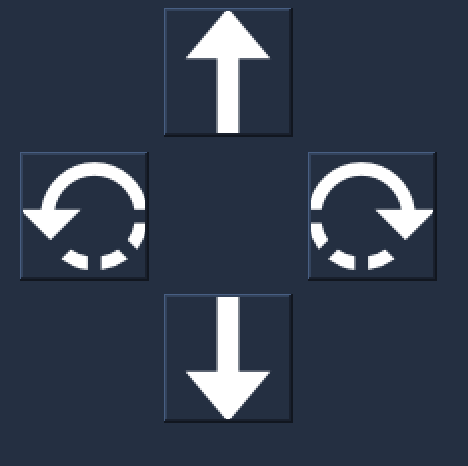
\includegraphics[width=0.3\textwidth]{ControlPanel}
\caption{Moving Control}
\label{moving control}
\end{figure}
The movement controls (Figure \ref{moving control}) are as follows:
\begin{itemize} \index{Movement control}
\item The button with the up arrow will send a forward command when the user clicks on it or presses the up arrow key on the keyboard.
\item The button with the down arrow will send a backward command when user clicks on it or presses the down arrow key on the keyboard.
\item The button with the left rotate arrow will send a left rotate command when the user clicks on it or presses the left arrow key on the keyboard.
\item The button with the right rotate arrow will send a right rotate command when user clicks on it or presses the right arrow key on the keyboard.  \index{Arrow keys - Control Panel}
\end{itemize}

\paragraph{Color Sensor movement}\label{COLORMOVE} \index{Color Sensor Movement}
\begin{figure}[!htb]
\centering
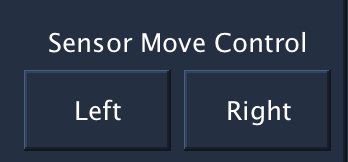
\includegraphics[width=0.4\textwidth]{SensorMove}
\caption{Color Sensor Move Control}
\label{color move}
\end{figure}
The color sensor movement controls (Figure \ref{color move}) are as follows:
\begin{itemize}
\item The left button will send a left move command to move the color sensor when the user clicks on it.
\item The right button will send a right move command to move the color sensor when the user clicks on it.
\end{itemize}

\paragraph{Emergency Stop} \label{EMERGENCYSTOP} \index{Emergency Stop}
\begin{figure}[!htb]
\centering

\includegraphics[width=0.2\textwidth]{EmergencyStop}
\caption{Emergency Stop}
\label{emergency stop}
\end{figure}
\begin{itemize}
\item The Emergency Stop button (Figure \ref{emergency stop}) will send an emergency stop command to the robot to stop the robot from movement immediately.
\end{itemize}

\subsubsection{Switch Panel} \index{Switch Panel}
\paragraph{Autonomous and Manual Switch}\label{CONTROLSWITCH}
Autonomous and Manual Switch (Figure \ref{control switch}) (R01 Manual Control and R02 Autonomous Control)\\
\begin{figure}[!htb]
\centering
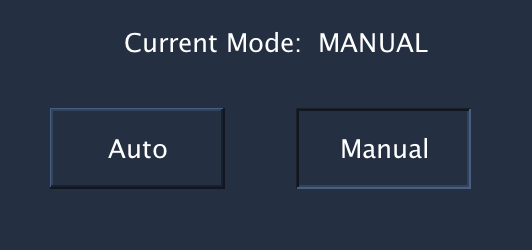
\includegraphics[width=0.3\textwidth]{AutoManualSwitcher}
\caption{Autonomous and Manual Switch}
\label{control switch}
\end{figure}
\begin{itemize} \index{Autonomous Mode Switching Button} \index{Manual Mode Switching Button}
\item When the manual button is selected, the robot will switch to the manual mode which allows the user to manually control the robot and enable the sending of robot movement commands.
\item When Auto button is selected, the robot will switch to the autonomous mode which enables self path finding of the robot and disables the sending of robot movement commands.
\item The current mode can be viewed on the status window.
\end{itemize}

\paragraph{Reset and Start New}\label{RESET}
\begin{figure}[!htb]
\centering
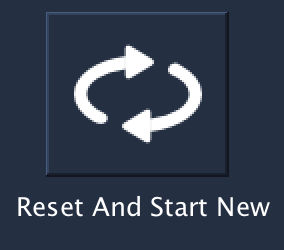
\includegraphics[width=0.2\textwidth]{Reset}
\caption{Reset and Start New}
\label{reset}
\end{figure}
\begin{itemize} \index{Reset map}
\item When the robot has reached the destination, the Reset and Start New button (Figure \ref{reset}) allows the User to reset the figures of map.
\end{itemize}

\subsubsection{Map Panel} \index{Map Panel}
\paragraph{Map display region}\label{MAPDISPLAY}
\begin{figure}[!htb]
\centering

\includegraphics[width=0.5\textwidth]{MapDisplay}
\caption{Map Display}
\label{map display}
\end{figure}
\begin{itemize} \index{Map Display Panel}
\item This region (Figure \ref{map display}) will display the map visualization by rendering the map data. It displays the robot position and map features. It also allows the user to modify the map by marking no go zones or creating destinations.
\end{itemize}

\paragraph{Map Editing Buttons}\label{MAPEDITING} \index{Edit map}
\begin{figure}[!htb]
\centering

\includegraphics[width=0.6\textwidth]{MapEditing}
\caption{Map Editing buttons}
\label{map editing buttons} \index{Map editing buttons}
\end{figure}
\begin{itemize}
\item The map editing buttons (Figure \ref{map editing buttons} are placed above the map display region. They have the functionalities to allow the user to modify the map.
\item When the "Create Destination" \index{Destination Create Button} button is clicked, it allows the user to create a destination by clicking a specific point on map. The text on this button will become "Confirm", and the user needs to click on it to confirm the destination.
\item When the "Load XML map" \index{XML Map Load Button} button is clicked, it allows the user to load the data of DTD.xml into the map structure. The DTD.xml will also be rendered and displayed to the user at the same time.
\item When the "Add No Go Zone" \index{No Go Zone Button} button is clicked, it allows the user to mark the NGZs on the map. This is done by using the mouse to drag a shape on the map display region. The text on this button will become "Confirm", and the user needs to click on it to confirm the NGZ.
\end{itemize}

\paragraph{Zoom In/Out} \label{ZOOM}
\begin{figure}[!htb]
\centering

\includegraphics[width=0.5\textwidth]{Zoom}
\caption{Zoom In/Zoom Out}
\label{zoom}
\end{figure}

\begin{itemize} \index{Zoom In}
\item One click on the "Zoom In" button (Figure \ref{zoom}) will enlarge the components displayed in the map by 10\%. \index{Zoom Out}
\item One click on the "Zoom Out" button (Figure \ref{zoom}) will narrow the components displayed in the map by 10\%.
\item When the map is zoomed in, user can click on the map to move the camera.
\end{itemize}

\paragraph{Save Map} \label{SAVEMAP}
\begin{figure}[!htb]
\centering

\includegraphics[width=0.3\textwidth]{Save}
\caption{Save Map}
\label{save map}
\end{figure}
\begin{itemize} \index{Save Map} \index{Export XML Button}
\item "Save Map" Button (Figure \ref{save map}) allows user to save the data of current map. All features of the map will be rendered into XML format.
\end{itemize}

\paragraph{Close button} \label{closeButton}
\begin{itemize}
\begin{figure}[!htb]
\centering

\includegraphics[width=0.2\textwidth]{Close.png}
\caption{Close Button}
\label{close button}
\end{figure} \index{Close program}
\item When the user clicks the "Close" button (Figure \ref{close button}), it will send command to close all the motor and sensor ports and then exit the program.
\end{itemize}


\newpage
\section{Building Connection}
\subsection{Cable} \index{Cable Connection instructions}
This is the simplest way to connect the robot. User needs to plug the USB cable on the robot USB port and the computer. The user can then launch the application and select "Cable" on connection screen. Upon successful connection, the main screen will pop up.

\subsection{Bluetooth} \index{Bluetooth Connection Instructions}
To connect the robot via Bluetooth, user needs to firstly turn on the Bluetooth on the computer then enter the Bluetooth setting on the EV3 brick. The brick should show your device name after searching. Then the user should confirm the device and there will be a pin shown on the brick screen. After entering this pin on the computer, the robot should connect to the computer. Then the user shall click Bluetooth on the connection screen. Upon successful connection, the main screen will pop up.
\subsection{WiFi} \index{WiFi Connection Instructions}
To connect the robot via WiFi, user needs to make sure the robot and the computer are connected to the same network via WiFi. There will be an assigned IP address displayed on brick. Then user shall click WiFi on the connection screen and enter the IP address displayed on the brick. Upon successful connection, the main screen will pop up.

\subsection{Frequent Problems On Connection} \index{Connection Problems}
In case the main screen didn't pop up and it stays on connection screen, It means the connection is not built. There are following ways to resolve this problem:
\begin{enumerate}
\item Try another connection method.
\item Check the message shown on the connection screen and make sure sensors and motors are correctly connected to the ports.
\item Enter brick setting, reset and try again.
\end{enumerate}
\newpage


\section{Manual Control}
\subsection{Switch to Manual control} \index{Manual Mode Control}
Manual control is the default mode at the launch of the application. Under this mode, User can control the robot manually. The buttons associated with manual control will be enabled. The user can click the buttons to control the movement of the robot in the control panel. Holding the button will make robot movement continuously.

\begin{figure}[!htb]
\centering
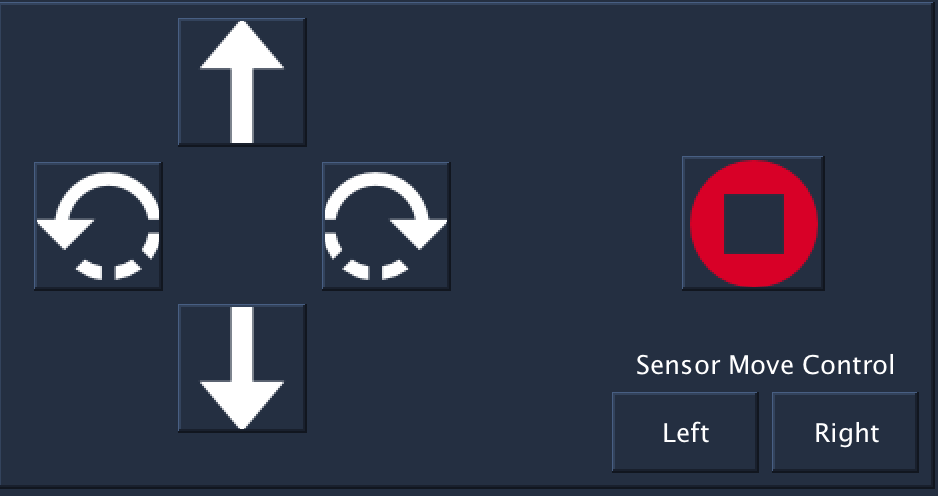
\includegraphics[width=0.5\textwidth]{RobotControlPanel.png}
\caption{Robot Control Panel}
\end{figure}

\subsection{Associated Key} \index{Arrow Keys - Manual Control}
\begin{itemize}
\item Moving forward -				Up Arrow Key
\item Moving Backward -   	Down Arrow Key
\item Turn Clockwise   -  		 Right Arrow Key
\item Turn Anti Clockwise -   	 Left Arrow Key
\item Emergency Stop -        Space
\end{itemize}

\textbf{NOTE} : The manual control buttons except Emergency stop will be disabled in Autonomous mode.

\newpage

\section{Autonomous}
\subsection{Switch to Autonomous} \index{Autonomous Mode Control}
The user can switch to Autonomous mode by clicking the "Auto" button in the switch panel. In this mode, the manual control buttons, except Emergency stop, will be disabled. The user can select a position on map display region by clicking to create a destination. If the path between the destination and the robot position is not blocked, the robot will automatically move to this destination through a shortest path.
\subsection{Setting up destination} \index{Destination Creation}
To set up a destination, the user needs to click the "Create Destination" button and select the destination (shown in Figure \ref{destination}) on the Map display region. After the first click on "create destination", the text of this button will be changed to "confirm" (shown on the Figure \ref{destination confirm}). User can click this button to confirm the destination position and then the robot will be moving to this position if the path is not blocked.

\begin{figure}[!htb]
\centering

\includegraphics[width=0.1\textwidth]{Destination.png}
\caption{Destination icon shown on the map display region}
\label{destination}is not blocked
\end{figure}

\begin{figure}[!htb]
\centering

\includegraphics[width=0.2\textwidth]{DestinationConfirm.png}
\caption{Destination confirm }
\label{destination confirm}
\end{figure}


\newpage
\section{Map Display}
\subsection{Display of Map Feature} \index{Map Display}
The map is updated regularly and the GUI displays the map in real time. When the robot detects the feature on the map, it will be shown on the map with the associated color:
\begin{itemize} \index{Map colors}
\item Border = Blue
\item Radiation = Green
\item Tracks = Purple
\item Craters = Black
\end{itemize}

\begin{figure}[!htb]
\centering
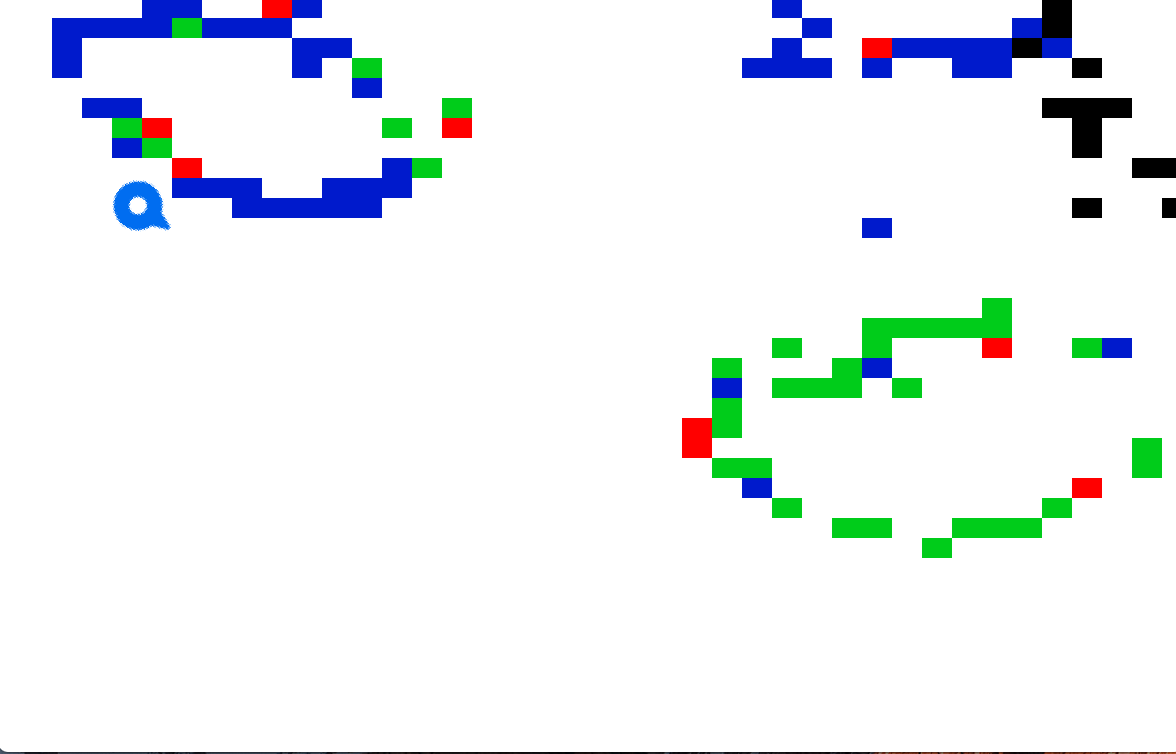
\includegraphics[width=0.7\textwidth]{ExampleOfMapDisplay.png}
\caption{Example of Map Display}
\end{figure}

\subsection{Create the No Go Zones} \index{No Go Zone Creation}
The user can create No Go zones by clicking the "Add No Go zone". It allows the user to drag a rectangular shape on the map and designate this region to be a No Go zone in the map structure. The user can add more than one No Go zones on the map.

\begin{figure}[!htb]
\centering
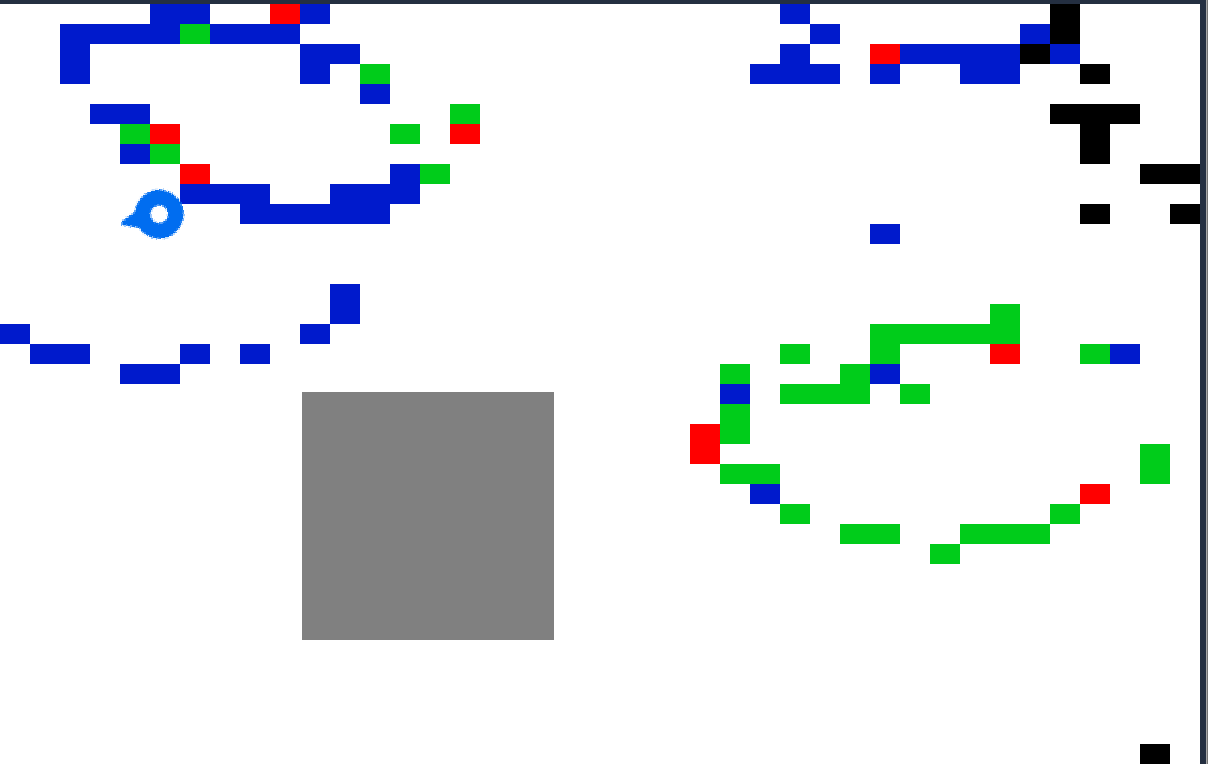
\includegraphics[width=0.7\textwidth]{ExampleOfNGZ.png}
\caption{Example of No Go Zone creation}
\end{figure}
\newpage
\subsection{Discard the Creations} \index{Map - Remove features}
The user can also disregard the creations on the map including destination by clicking the "reset" button on the switch panel (refer to Section \ref{RESET}).
\subsection{XML Import} \index{XML Import}
User can import the XML into map structure by clicking "import XML file" on map editing section (refer to Section \ref{MAPEDITING}).
\subsection{XML Export} \index{XML Export}
User can export the XML into map structure by clicking "save the map" on map display control section (refer to Section \ref{SAVEMAP}).

\printindex

\end{document}
